\chapter[General introduction]{General introduction: molecular microbial ecology of Antarctic lakes}
\label{ch:intro}

%Coauthorship-----------------------------------------------------------------------------------

\section*{Co-authorship statement}
\addcontentsline{toc}{section}{Co-authorship statement}

Sections of this chapter has been published as:\\

David Wilkins, \textbf{Sheree Yau}, Timothy Williams, Michelle Allen, Mark V. Brown, Matthew Z. DeMaere, Federico M. Lauro and Ricardo Cavicchioli. 
Key Microbial Drivers in Antarctic Aquatic Environments. \\
\textit{\underline{FEMS Microbiology Reviews}} 
(doi: 10.1111/1574-6976.12007), 2012.\\

I contributed the section of the publication entitled \emph{Antarctic lakes} excluding the subsection, \emph{Microbial mats as microcosms of Antarctic life}.
This material appears in section~\ref{in:mol} \emph{Molecular approaches used in Antarctic lake systems}, section~\ref{in:insights} \emph{Molecular insights into Antarctic lakes} and section~\ref{in:pcrlimits} \emph{limitations of taxonomic surveys} of this introduction.
\newpage

%-----------------------------------------------------------------------------------------------

\section{Introduction}
Antarctica is a ``frozen desert'' of constant low temperature, little precipitation and subject to the polar light cycle where only specially adapted organisms can survive.
The continent is covered by ice up to 4 km thick that spans 13.8 million km$^2$.
A tiny 0.32\% of the land area is ice-free, most of which consists of exposed rocky peaks or nunataks such as in the Ellsworth, the Transantarctic and the North Victoria Land Mountains. %figure of continent
Only 1--2\% of that ice-free land is found in coastal oases; however, it is these regions where Antarctic life is concentrated \cite{Hodgson2012}.

They are breeding sites for large animals such as seals, penguins and sea birds and some of the only locations where plants and lichens are found.
Coastal oases are also distinguished by the presence of hundreds of lakes and ponds.
Life in these lakes is microbially dominated with few, if any, metazoan inhabitants \cite{Laybourn-Parry1997} making them ideal locations to study Antarctic microbiota. 
The lakes span a continuum of environmental factors such as salinity and are ``natural laboratories'' to examine adaptations to a property of interest. 
They are also ideal model ecosystems as they are largely isolated with a close relation between species and function.

This introduction will describe the Antarctic lakes, their microbiology and review molecular-based Antarctic microbiological research on the lakes.
As this thesis focused on two lakes in the Vestfold Hills, emphasis will be given to describing research from this study site.

%---------------------------------------------------------------------------------------------

\section{Antarctic lakes}
%create a map of the regions you want to describe, like in the review paper.
In Antarctica, perenially available liquid water is found predominantly in lakes. 
These lakes span a wide range of physical and chemical properties from freshwater to hypersaline and constantly ice-covered to melted.
Some are permanently stratified and termed meromictic if they thaw seasonally, or amictic if they are always ice-covered.
Stratified lakes provide a unique opportunity to describe microbial populations along chemical gradients within a single water body. 
Most lakes are ice-covered for most of the year making them effectively isolated, and some may be truly closed systems if ice-cover is permanent.
The age of water varies considerably; for example, outflow of subglacial water at Blood Falls is estimated to be 1.5 million years old \cite{Mikucki2009} while water from Lake Miers is less than 300 years old \cite{Green1988}. 
Overall, there are two main Antarctic lake types: those bound by ice, comprising subglacial; epiglacial and supraglacial lakes, and those bound by rock.

\subsection{Ice-bound lakes}
Subglacial lakes are pools of water beneath an ice sheet that form as the pressure of glacier flow against bedrock melts the ice at the interface. 
They are prevalent in Antarctica with at least 145 identified \cite{Siegert2005}.
The largest of these is Lake Vostok, which is 240 km long, 50 km wide and up to 1 km deep \cite{Siegert2001}.
Here the pressure is an extreme 340 atmospheres \cite{Siegert2001}.
These lakes are found dotted around the continent generally, under the continental ice shelf \cite{Siegert2001}.%ref Pearce 2009.

Epiglacial lakes are similarly formed in the boundary between rock and ice, but where rock is exposed, such as where a glacier front contacts a mountain side.
They are potentially the most common lake type as they can occur where ever there is rock and thus are both inland and on the coast \cite{Hodgson2012}. % gibson2006?
These lakes can be highly changeable as they are subject to glacial movements and meltwater inputs.
As a result, they can be short-lived, but many examples are thousands of years old, such as the .

Pockets of water can be also be found on top of glaciers. 
One example is cryoconite holes, which originate from the heat absorbed by dark dust melting small depressions on the glacier surface. 
These are extremely interesting systems with massive ranges in pH and chemistry.
Supraglacial lakes with more substantial volumes of waters also occur.
However, all of them tend to be ephemeral lasting only during the summer months.

\subsection{Rock-bound lakes}
These lakes are of water trapped in exposed rocky basins.
Look up the Mountain lakes. %How are they formed. Where are they? Some examples.

By far the majority of lakes are found in the coastal oases. %How many?
Most of these lakes were formed when the retreat of the continental ice-shelf lead to isostatic uplift of the land \cite{Burton1981}. %check ref
As a result, the majority of lakes in the coastal oases are composed of relic seawater and are predominantly saline or hypersaline \cite{Burke1988}.
In the latter, salinity is high due to concentrated by ablation (evaporation and sublimnation). %ref 
Lakes closer to the coastline may still occasionally experience marine inputs. %ref
Epishelf lakes are a type of lake unique to coastal regions.

Freshwater lakes near the continental ice shelf were likely already above sea-level as the ice receded and are not of marine origin \cite{Bronge1996}. %Laybourn-Parry1992?
Other freshwater lakes were originally marine-derived but have been flushed fresh by glacial meltwater \cite{Pickard1986}.
All lakes may receive water inputs from precipitation, from the ice-shelf and glacial melt streams \cite{Burton1981}. 
This can cause freshwater to seasonaly overlay some saline lakes as the ice-cover thaws.
The chemistry of the exposed lakes is very much influenced by the water balance from local geographic and climatic conditions which leads them to have different physical and chemical properties.

\section{Coastal oases}
Coastal oases are the best studied systems as they are the most hospitable sites for research stations.
Those where lakes are found fringe the Antarctic continent.
%ages of the coastal oases.
%paleogeography of coastal oases
In East Antarctica these include the Vestfold Hills, Bunger Hills, Larsemann Hills, Syowa Oasis, Schirmacher Oasis, Grearson Hills and McMurdo Dry Valleys.
In West Antarctic, the Antarctic Peninsula, the sub-antarctic islands and maritime islands house multiple lakes. 
Of these locations, the best studied lake systems are those of the McMurdo Dry Valleys, The Vestfold Hills and the subantarctic islands.
%refer to table or map of the region
%How long have people done research on these lakes?

%--------------------------------------------------------------------------------------------

\section{The Vestfold Hills, East Antarctica}
The Vestfold Hills \figref{fig:vestfold_map} is a ice-free region of approximately 400 km$^2$ on the eastern shore of the Prydz Bay, East Antarctica in the Australian Antarctic Territory \cite{Gibson1999}.
\begin{figure}
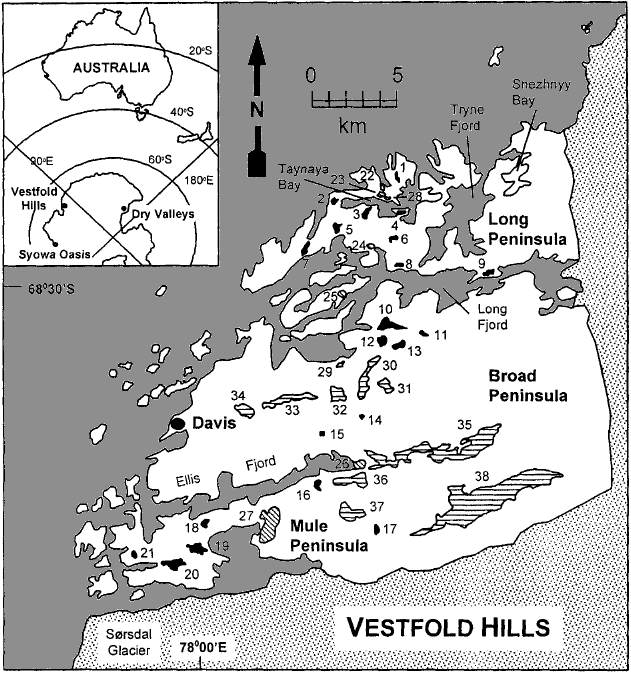
\includegraphics{intro_figures/vestfold_map.png}
\caption[Map of the Vestfold Hills]{A map of the Vestfold Hills showing fjords, bays and lakes (numbered). The Southern Ocean is shown in grey, meromictic lakes coloured in black, seasonally isolated lakes and basins are striped and the continental ice-shelf is stippled. Inset is the position of the Vestfold Hills relative to Australia and to the Antarctic coastal oases. The lakes are: (1) unnamed lake 2, (2) Organic Lake, (3) Pendant Lake, (4) Glider Lake, (5) Ace Lake, (6) unnamed lake 1, (7) Williams Lake, (8) Abraxas Lake, (9) Johnstone Lake, (10) Ekho Lake, (11) Lake Farrell, (12) Shield Lake, (13) Oval Lake, (14) Ephyra Lake, (15) Scale Lake, (16) Lake Anderson, (17) Oblong Lake, (18) Lake McCallum, (19) Clear Lake, (20) Laternula Lake and (21) South Angle Lake. Map image is from \citet{Gibson1999} with some minor modifications.}
\label{fig:vestfold_map}

\end{figure}

The region is made up of three large peninsulae, Broad, Mule and Long Peninsula, separated by fjords connected to the sea.
Some of these are large, such as Ellis Fjord, which is 10 km long, up to 100 m deep and has become a stratified system due to its restricted opening to the ocean \cite{Burke1988}.
The region was formed approximately 10,000 years ago in the early Holocene as the continental ice receded and the rocky peninsulae rose above sea-level \cite{Zwartz1998}. 

The Vestfold Hills were first sighted and named in 1935 \cite{Law1959}.
Only intermittent expeditions occurred in the area until the establishment of Davis Station (68$^{\circ}$33$'$S, 78$^{\circ}$15$'$E) in 1957 \cite{Law1959}. 
A continuous presence has been maintained since. %sometime
There Vestfold Hills region was immediately noted for its extensive ice-free land and the numerous lakes \cite{Johnstone1973}.

The Australian Antarctic Data Centre lists more than 3,000 water bodies mapped in the Vestfold Hills, ranging in area from 1 to 8,757,944 m$^2$. %check this fact.
More than 300 lakes and ponds have been described, including approximately 20\% of the world's meromictic lakes \cite{Gibson1999}. %check this fact.
These are of particular interest because the anoxic bottom waters help preserve a paleogeological record in the sediments.
This can tell us about the region and particularly climatic changes.
Stratified lakes provide a unique opportunity to describe microbial populations along chemical gradients, but within a single water body. 
%Show a map of some of the main lakes in the Vestfold Hills
%Nutrient status? (see Burton 1981) temperature? weather? major ions? (see Burton1981). recorders of climate change in the sediment and in the location of the chemocline,what occurs in each zone


\subsection{Biology of the Vestfold Hills}

The Vestfold Hills is an oasis for life.
Here is a breeding ground for seabirds, penguins and seals.
Plant life exists as mosses and lichens.
Most of the life is microbial.


%------------------------------------------------------------------------------------------

\section{Cultivation and microscopy-based Antarctic microbiology}

Microbiological studies have been conducted in the lakes regions since X.
These were conducted using cultivation and/or microscopy-based identification and quantification. 
\emph{Eucarya} were identified with microscopy based approaches.
For \emph{Bacteria}, only those that could be isolated, distinguished by morphology or biochemical tests were readily identifiable.
Were Archaea known?

\subsection{Viruses}
%Any cultured viruses?
As obligate parasites, culturing viruses is made problematic by the need to have a susceptible host in culture.
Furthermore, host specificity can be extremely narrow so any assessment of viral diversity by cultivation is highly limited.
This is compounded by the logistical constraints of conducting field work in the Antarctic.

Most studies of Antarctic viruses have been confined to diversity analyses based on the electron micrographs of \ac{VLP} morphotypes or visibly infected cells. 
Electron micrographs are able to distinguish to some extent tailed bacteriophages such as myo- sipho- and podo- viruses from one another due to tail morphology.
For tailess viruses with icosohedral symmetry, morphology alone provides hardly any distinguishing features apart from capsid size.
Other metrics used to assess viruses in the environment include enumeration, virus to bacteria ratios, visibly infected cells and viral production rates.

Overall, pioneering work on viruses has made several noteworthy observations. 
\begin{enumerate}
\item Viruses are possibly more abundant in high latitude lakes than lower latitude.
\item Burst sizes of viruses are lower in high latitude lakes than in low latitude.
\item Viral abundance appears to correlate positively with salinity.
\item As food chains in Antarctic Lakes are truncated, viruses may play an increased importance in Antarctic lakes, particularly in increasing secondary production through the microbial loop.
\item %viral to bacterial ratios???
\item %viral production.
\end{enumerate}
In the absence of metazoan grazers, viruses are hypothesized to play an increased role in the microbial loop in Antarctic systems \cite{Kepner1998} and as drivers of microbial evolution \cite{Anesio2011}. 
This idea has been supported by microscopy-based observations of viral density, virus to bacteria ratios and infection rates that are different in Antarctic lakes than lower latitude systems \cite{Laybourn-Parry2001, Madan2005, Laybourn-Parry2007, Sawstrom2007}. 
Cold environments are hypothesized to be a `hotspot' of viral diversity.
However, molecular methods are required to validate this claim.

%------------------------------------------------------------------------------------------

\section{Molecular approaches used in Antarctic lake systems}
\label{in:mol}
The majority of molecular-based studies of Antarctic aquatic microbial communities have made use of \ac{PCR} amplification of \ac{SSU} sequences to survey the diversity of \emph{Bacteria}
 and in some cases \emph{Archaea} and \emph{Eucarya} \tabref{tab:pcr_lakes}.
Microbial composition has been determined by cloning and sequencing of \ac{rRNA} gene amplicons exclusively 
\cite{Bowman2000a, Bowman2000, Gordon2000, Christner2001, Purdy2003, Karr2006, Matsuzaki2006, Kurosawa2010, Bielewicz2011}, 
although most studies have also made use of \ac{DGGE} to provide a molecular ``fingerprint'' of the community 
\cite{Pearce2003a, Pearce2003b, Karr2005, Pearce2005a, Pearce2005b, Unrein2005, Glatz2006, Mikucki2007, Mosier2007, Schiaffino2009, Villaescusa2010}.
Functional genes have also been targeted using polymerase chain reaction (PCR) amplification to assess the potential of biochemical processes occurring, such as nitrogen fixation \cite{Olson1998}, 
ammonia oxidation \cite{Voytek1999}, anoxygenic photosynthesis \cite{Karr2003}, and dissimilatory sulfite reduction \cite{Karr2005, Mikucki2009}. %add in new studies
\begin{landscape}

\begin{table}
\caption[PCR-based studies of Antarctic Lakes]{Studies of Antarctic Lakes that have made use of PCR amplification and sequencing of marker genes.}
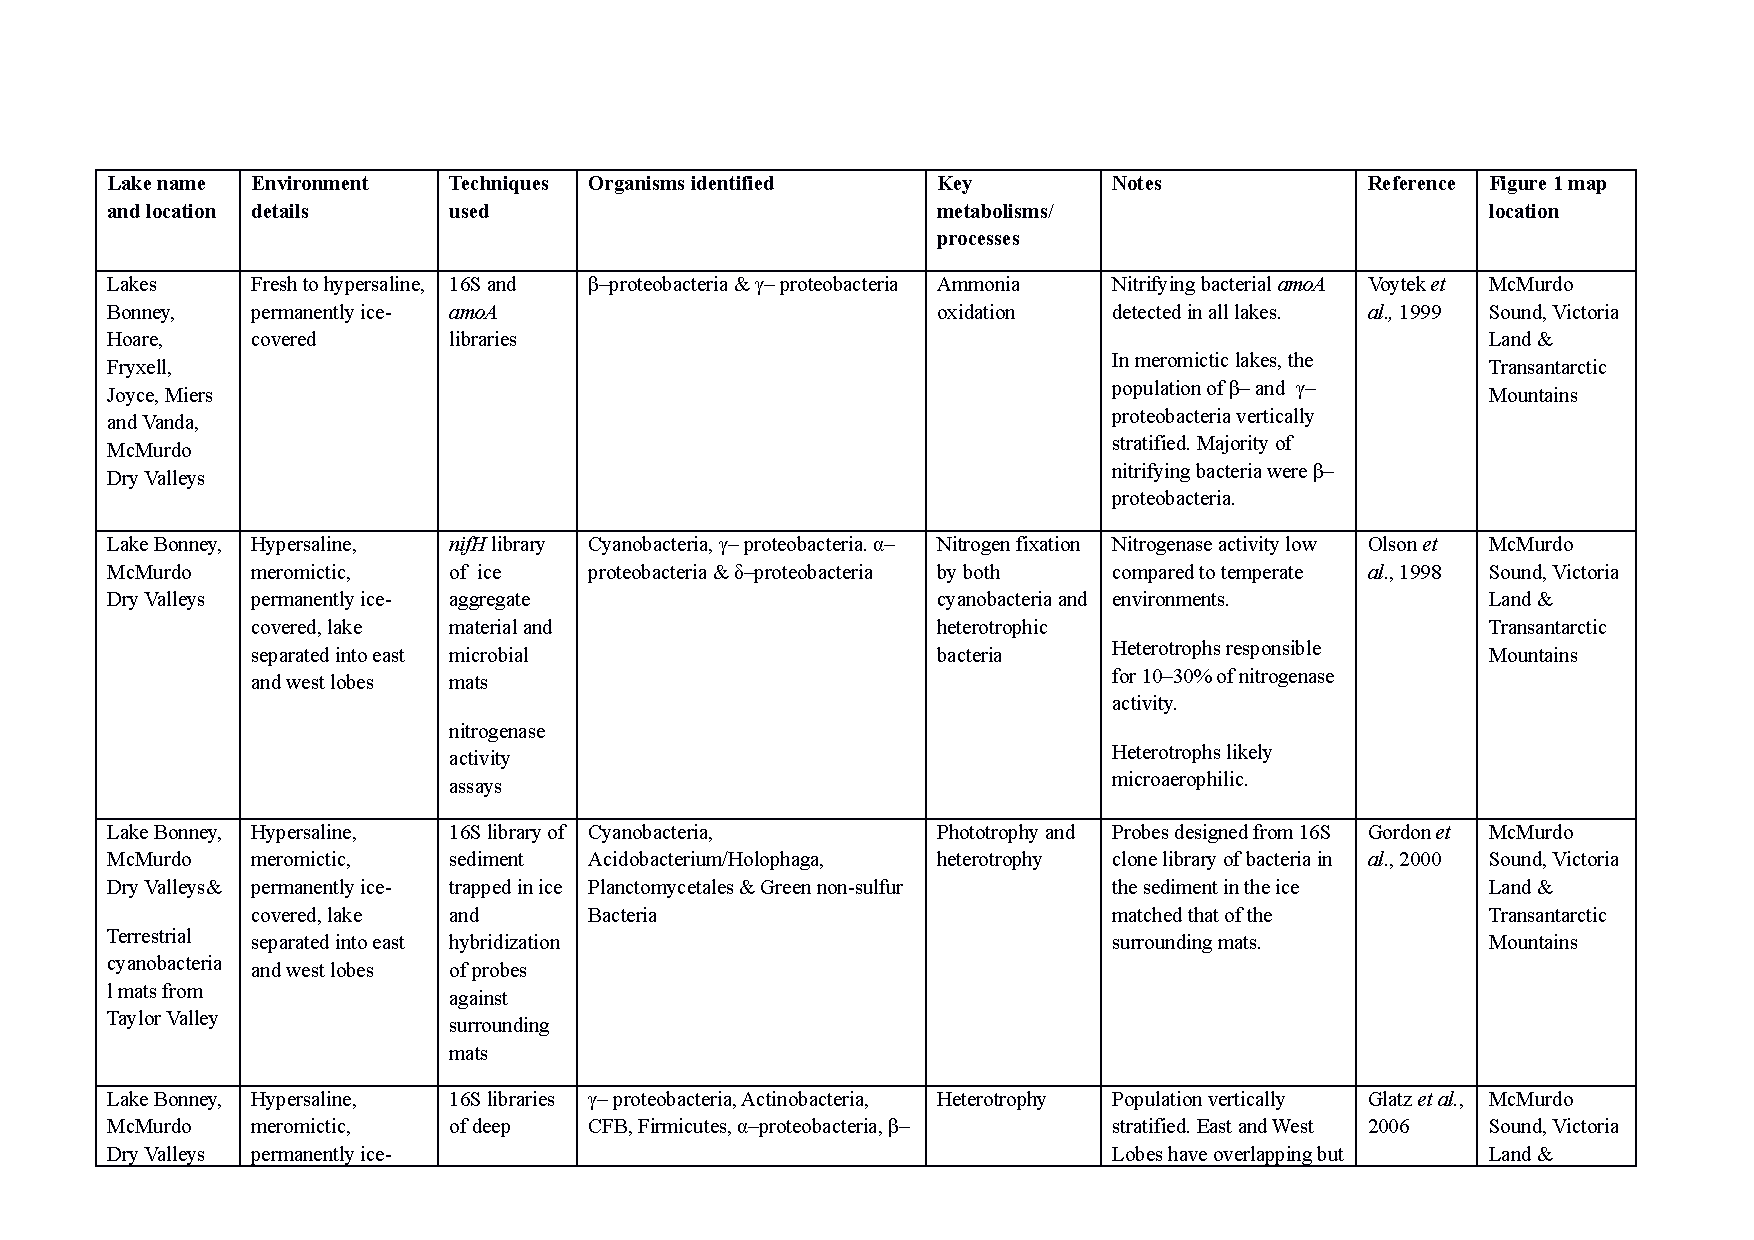
\includegraphics{intro_figures/molecular_studies_lakes.pdf}
\label{tab:pcr_lakes}
\end{table}

\end{landscape}


%-----------------------------------------------------------------------------------------

\section{Insights from Antarctic molecular studies}
\label{in:insights}
\subsection{Bacterial diversity: adaptation to unique physical and chemical conditions}
The vast majority of molecular studies of Antarctic lakes have focused on bacteria.
Consistent with the wide range of physical and chemical properties of Antarctic lakes, a large variation in species assemblages have been found.
While exchange of microorganisms must be able to occur between lakes that are in close vicinity to each other, 
the picture that has emerged from the data to date is that microbial populations are relatively unique to each type of isolated system. 
Nonetheless, certain trends in bacterial composition are also apparent.

Focusing on the similarities, lakes of equivalent salinities tend to have similar communities.
Hypersaline lakes from the Vestfold Hills \cite{Bowman2000} and McMurdo Dry Valleys \cite{Glatz2006, Mosier2007} were all dominated by \emph{Gammaproteobacteria} and members of the Bacteroidetes
 as well as harboring lower abundance populations of \emph{Alphaproteobacteria}, \emph{Actinobacteria}, and \emph{Firmicutes}.
The surface waters of saline lakes resemble marine communities dominated by \emph{Bacteroidetes}, \emph{Alphaproteobacteria} and \emph{Gammaproteobacteria},
 but divisions such as \emph{Actinobacteria} and specific clades of \emph{Cyanobacteria} have been found to be overrepresented compared to the ocean \cite{Lauro2011}.
Sediments from saline lakes in the Vestfold Hills \cite{Bowman2000a} and Nuramake-Ike in the Syowa Oasis \cite{Kurosawa2010} were very similar, 
containing in addition to the surface clades, \emph{Deltaproteobacteria}, \emph{Planctomycetes}, \emph{Spirochaetes}, \emph{Chloroflexi} (green non-sulphur bacteria), \emph{Verrucomicrobia} and representatives of candidate divisions.
Plankton from freshwater lakes were characterized by an abundance of \emph{Betaproteobacteria}, although \emph{Actinobacteria}, \emph{Bacteroidetes}, \emph{Alphaproteobacteria} and \emph{Cyanobacteria} were also prominent \cite{Pearce2003a, Pearce2005a, Pearce2005b, Schiaffino2009}. 

\subsubsection{Bacterial diversity defined by nutrients}
Differences in bacterial community structure are also influenced by nutrient availability.
In studies of freshwater lakes in the Antarctic Peninsula and the South Shetland Islands, cluster analysis of \ac{DGGE} profiles grouped together lakes of similar trophic status 
\cite{Schiaffino2009, Villaescusa2010}.
Most of the variance in community structure could be explained by related chemical parameters such as phosphate and dissolved inorganic nitrogen.
Similarly, three freshwater lakes, Moss, Sombre and Heywood on Signy Island are alike except that Heywood Lake is enriched by organic inputs from seals.

Bacterial composition in each lake changed from winter to summer and this was again correlated to variation in physico-chemical properties \cite{Pearce2005a}. 
The bacterial population of Heywood Lake had shifted from a dominance of \emph{Cyanobacteria} towards a greater abundance of \emph{Actinobacteria} and marine \emph{Alphaproteobacteria} \cite{Pearce2005b}.
This hints at a link between a copiotrophic lifestyle in the Heywood Lake \emph{Actinobacteria} and inhibition of Antarctic freshwater \emph{Cyanobacteria} by eutrophication. 
This type of study exemplifies how inferences can be made about taxa and function by examining population changes over time and over gradients of environmental parameters.

\subsubsection{Bacterial biogeography}
The relative isolation and diverse chemistries of the lakes facilitates biogeographical and biogeochemical studies. 
The anoxic and sulfidic bottom waters of some meromictic lakes form due to a density gradient that precludes mixing. 
Although sedimentation from the upper aerobic waters may occur, 
there is little opportunity for interchange of species with the bottom water of lakes allowing for greater divergence in community composition as nutrients can become depleted 
and products of metabolism can accumulate.
As a result, distinct distributions of bacterial groups can inhabit these strata, and different types of microorganisms can be found in equivalent strata in different lakes. 
A good example of this is the presence of common types of purple sulphur bacteria (\emph{Chromatiales})and \ac{GSB}(\emph{Chlorobi}) 
in some meromictic lakes and stratified fjords in the Vestfold Hills \cite{Burke1988},
compared to diverse purple non-sulphur bacteria in Lake Fryxell in Victoria Land \cite{Karr2003}. 
%Check if these aren't Roseobacters
In Lake Bonney, the east and west lobes harbor overlapping but distinct communities in the suboxic waters \cite{Glatz2006}.
The east lobe was dominated by \emph{Gammaproteobacteria} and the west lobe by \emph{Bacteroidetes}, illustrating how divergent communities can form from the same seed population. 
In contrast, ice communities are more readily dispersed by wind, aerosols and melt-water. 
16S rRNA gene probes designed from bacteria trapped in the permanent ice-cover of Lake Bonney hybridized to microbial mat libraries sourced up to 15 km away \cite{Gordon2000}.
This demonstrates how a single lake may encompass microorganisms that are geographically dispersed, while also harboring others that have restricted niches and are under stronger selection pressure.


\subsubsection{Bacterial diversity of Lake Vostok}
Subglacial systems, such as Lake Vostok, have been isolated from the open environment for hundreds of thousands to millions of years \cite{Siegert2001}.
As a result they provide a reservoir of microorganisms that may have undergone significant evolutionary divergence from the same seed populations that were not isolated by the Antarctic ice cover. 
Lake Vostok is approximately 4 km below the continental ice-sheet making it extremely difficult to determine suitable means for accessing the lake without inadvertently contaminating it with biological
 or chemical matter \cite{Inman2005, Wingham2006, Lukin2011, Gramling2012, Jones2012}. 
To date, molecular microbial studies have concentrated on the accretion ice above the ice-water interface \cite{Priscu1999, Christner2001}.
Accretion ice has been found to contain a low density of bacterial cells from \emph{Alphaproteobacteria}, \emph{Betaproteobacteria}, \emph{Actinobacteria} and \emph{Bacteroidetes} divisions closely allied to other cold environments.
Molecular signatures of a thermophilic \emph{Hydrogenophilus} species were also identified in accretion ice 
raising the possibility that chemoautotrophic thermophiles were delivered to the accretion ice from hydrothermal areas in the lake’s bedrock \cite{Bulat2004, Lavire2007}.
However, interpretation of results from samples sourced from the Lake Vostok bore hole are very challenging as it is difficult to differentiate contaminants from native Vostok microorganisms.
From a study that assessed possible contaminants present in hydrocarbon-based drilling fluid retrieved from the Vostok ice core bore hole, 
six phylotypes were designated as new contaminants \cite{Alekhina2007}. 
Two of these were \emph{Sphingomonas} phylotypes essentially identical to those found in the accretion ice-core \cite{Christner2001},
 which raises question about whether bacterial signatures identified from the ice-cores are representative of Lake Vostok water,
 and further highlights the ongoing problem of causing forward contamination into the lake.

\subsection{\emph{Archaea}: methanogens and haloarchaea}
\emph{Archaea} have been detected mainly in anoxic sediments and bottom waters from lakes that range in salinity from fresh to hypersaline, 
and those with known isolates are affiliated with methanogens or haloarchaea \cite{Bowman2000, Bowman2000a, Purdy2003, Kurosawa2010, Lauro2011}.
%relate how this is different to marine deep waters where Crenarchaea are abundant.
Anoxia allows for the growth of methanogenic \emph{Archaea} that mineralize fermentation products such as acetate, H$_2$ and CO$_2$ into methane, thereby performing an important step in carbon cycling.
The acetoclastic methanogens thrive in environments where alternative terminal electron acceptors such as sulfate and nitrate have been depleted. 
%This may be why there are none in Organic Lake as there is still sulfate.

One example of this is Lake Heywood where methanogenic \emph{Archaea} were found to comprise 34\% of the total microbial population in the freshwater sediment, 
the majority of which were \emph{Methanosarcinales} which include acetate and C1-compound utilizing methanogens \cite{Purdy2003}. 

In general, archaeal populations appear to be adapted to their specific lake environment.
Sediments from saline lakes of the Vestfold Hills were inhabited by members of the \emph{Euryarchaeota} typically found in sediment and marine environments 
with the phylotypes differing between the lakes examined \cite{Bowman2000a}. 
While a phylotype similar to \emph{Methanosarcina} was identified, the majority were highly divergent. 
Similarly, \emph{Methanosarcina} and \emph{Methanoculleus} were detected in Lake Fryxell but other members of the \emph{Euryarchaeota} and \emph{Crenarchaeota} (a single sequence) were divergent, 
clustering only with marine clones \cite{Karr2006}. 
Based on the lake chemical gradients and the location of these novel phylotypes in the water column the authors speculated these archaea may be have alternative metabolisms such as anoxic methanotrophy or sulphur-utilization. 

In sediments from Lake Nurume-Ike in the Langhovde region, 205 archaeal clones grouped into three phylotypes, 
with the predominant archaeal clone being related to a clone from Burton Lake in the Vestfold Hills, while the other two did not match to any cultivated species \cite{Kurosawa2010}. 
In hypersaline lakes where bottom waters do not become completely anoxic, methanogens are not present and \emph{Archaea} have extremely low abundance. 
For example, only two archeael clones of the same phylotype were recovered from deep water samples from Lake Bonney \cite{Glatz2006}, 
and Organic Lake in the Vestfold Hills had an extremely low abundance of archaeal clones related to \emph{Halobacteriales} \cite{Bowman2000}. 
In contrast to these stratified hypersaline lakes, the microbial community in the extremely hypersaline Deep Lake is dominated by haloarchaea \cite{Bowman2000}. 
Many of the clones identified from Deep Lake are similar to \emph{Halorubrum} (formerly \emph{Halobacterium}) \emph{lacusprofundi} which was isolated from the lake \cite{Franzmann1988}. 

\subsection{\emph{Eucarya} perform multiple ecosystem roles}

Single-celled \emph{Eucarya} are important members of Antarctic aquatic microbial communities.
In many Antarctic systems, eucaryal algae are the main photosynthetic organisms and in others, only heterotrophic protists occupy the top trophic level. 
As eucaryal cells are generally large with characteristic morphologies, microscopic identifications have been used. 
However, microscopy is unable to classify smaller cells such as nanoflagellates with high resolution, although these may constitute a high proportion of algal biomass.
For example, five morphotypes of \emph{Chrysophyceae}, evident in Antarctic lakes were unidentifiable by light microscopy but were able to be classified using \ac{DGGE} and DNA sequencing \cite{Unrein2005}.
Consistent with this, molecular studies specifically targeting eucaryal diversity \cite{Unrein2005, Mosier2007, Bielewicz2011} have identified a much higher level of diversity than previously suspected,
 and the studies have discovered lineages not previously known to be present such as silicoflagellates of the family \emph{Dictyochophyceae} \cite{Unrein2005} and fungi \cite{Mosier2007, Bielewicz2011}.

Most \emph{Eucarya} in Antarctic lakes are photosynthetic microalgae that are present in marine environments with a wide distribution including chlorophytes, haptophytes, cryptophytes and bacillariophytes.
Molecular methods have afforded deeper insight into the phylogenetic diversity within these broader divisions and have revealed some patterns in their distribution. 
Using 18S \ac{rRNA} gene amplification and \ac{DGGE}, the same chrysophyte phylotypes were identified in lakes from the Antarctic Peninsula and King George Island 
despite being 220 km apart \cite{Unrein2005} indicating these species may be well-adapted to Antarctica or highly dispersed.
Similarly, an unknown stramenopile sequence was detected throughout the 18S \ac{rRNA} clone libraries of Lake Bonney 
demonstrating a previously unrecognized taxon occupied the entire photic zone in the lake \cite{Bielewicz2011}. 
In constrast, other groups showed distinct vertical and temporal distributions with cryptophytes dominating the surface, 
haptophytes the midwaters and chlorophytes the deeper layers during the summer while stramenopiles increased in the winter \cite{Bielewicz2011}. 
Further studies are necessary to determine the basis for apparent specific adaptations of some species to particular lakes or lake strata, and for the cosmopolitan distribution of others.
Here, molecular based research of the kind that has been applied to bacteria such as functional gene surveys will undoubtedly help answer these questions.
%add in new studies of photosynthetic genes

\subsection{Functional gene studies of Antarctic lakes}

\subsection{Integrative studies to derive whole ecosystem function}
%----------------------------------------------------------------------------------------------------------------------


\section{Limitations of taxonomic surveys}
\label{in:pcrlimits}

Inferring functional potential from taxonomic surveys can be problematic due to species or strain level differences in otherwise related bacteria.
For example, the majority of the \emph{Gammaproteobacteria} in hypersaline lakes were relatives of \emph{Marinobacter} suggesting that this genus is particularly adapted to hypersaline systems
\cite{Bowman2000a, Glatz2006, Matsuzaki2006, Mosier2007}.
Nonetheless, \emph{Marinobacter} species from different lakes appeared biochemically distinct
 as isolates from hypersaline lake Suribati-Ike were all able to respire \ac{DMSO} but not nitrate \cite{Matsuzaki2006}. 
In contrast, those from the west lobe of Lake Bonney were all able to respire nitrate \cite{Ward1997}. 
Interestingly, in the east lobe of the same lake, nitrate respiration was inhibited although a near-identical \emph{Marinobacter} phylotype was present; 
it was speculated that the inhibition may have been caused by an as yet unidentified chemical factor \cite{Ward2005, Glatz2006}. 

This also applies to \emph{Eucarya}, as the influence of flagellates on ecosystem function is not necessarily clear-cut as they can simultaneously inhabit several trophic levels. 
For instance, in Ace Lake the mixotrophic phytoflagellate \emph{Pyramimonas gelidocola} derives a proportion of its carbon intake through bacterivory \cite{Bell2003} 
but in the nearby Highway Lake, it uptakes dissolved organic carbon \cite{Laybourn-Parry2005}. 
This again illustrates potential limitations for deriving ecosystem level functions from taxonomic studies alone, even with taxa that appear physiologically straightforward. 

%More examples eg. limitations of functional gene surveys due to horizontal gene transfer.


%--------------------------------------------------------------------------------------------------------------------

\section{`-omics' approaches}
Metagenomic studies have assessed both the taxonomic composition and genetic potential of lake communities, and in some cases have linked function to specific members of the community 
\cite{Lopez-Bueno2009, Ng2010a, Lauro2011, Yau2011, Varin2012}.
When coupled with functional ``omic'' techniques (to date metaproteomics has been applied, but not metatranscriptomics or stable isotope probing), 
information has also been gained about the genetic complement that has been expressed by the resident populations \cite{Ng2010a,Lauro2011}.
More detailled description of the advances of `-omics' approaches is detailed in the introduction of chapter 2.
%Refer forward.

Metagenomics has enabled unprecedented insight into viral diversity and ecology by permitting more precise classification, information on genetic content and discovery of novel species. 
Metagenomic analysis of the viriome of the freshwater Lake Limnopolar, Livingston Island uncovered the greatest depth of viral diversity of any aquatic system to date \cite{Lopez-Bueno2009}.
Representatives from 12 viral families were detected, but unlike the two previous viromes that had been published at that time using comparable techniques, ssDNA viruses and large dsDNA viruses that putatively infect eucarya were the dominant viral types rather than bacteriophages. 
The ssDNA viruses were related to circoviruses, geminiviruses, nanoviruses and satellites; viruses previously only known to infect plants and animals indicating they are much more diverse than previously suspected and may constitute new viral families. 
Samples taken in summer showed a shift in the viral community composition towards phycodnaviruses similar to Ostreococcustauri virus, OtV5. 
This shift potentially reflects an increase in the host algae that are stimulated to bloom by the increased light availability.

Understanding of Antarctic viral diversity and ecology is still in its early days as a complete viral survey is problematic due to the lack of a universal viral gene or even universal genetic material. 
Furthermore, the enormous depth of viral diversity remains largely unsampled so most viral sequences have no significant similarity to sequence data repositories \cite{Lopez-Bueno2009}. 
What is clear is that viruses perform a crucial role in shaping community structure, driving host evolution, contributing to the dissolved nutrient pool, and understanding them is essential to understanding ecosystem function \cite{Danavoro2011}. 
%-----------------------------------------------------------------------------------------------------------------

\section{Objectives}
This study aimed to use a primarily metagenomic approach complemented with microscopy and metaproteomics to gain an integrative understanding of whole ecosystems.
Ace Lake and Organic Lake were chosen as the study sites because as meromictic systems, differences in the microbial population can be examined across vertical gradients, they are also largely isolated, as marine-derived systems, adaptation of marine microbiota to lake system can be examined, they are sites of moderate diversity and may be reservoirs of unknown taxa.
Using this methodology, not only can the taxonomic composition of the lakes be determined but also the functional potential of the microbial population and insight into the active members of the community.
The objectives of the research were:

\begin{enumerate}
\item 
  To develop complementary analyses to metagenomic analysis.

\item
  To determine the microbial and viral composition of the lake communities and their functional potential.

\item
  To identify the genes expressed by the community.

\item
  To reconstruct genomic information of dominant taxa of interest.

\item
  To integrate environmental and biological data to model the lake microbial interactions and geochemical processes.

\end{enumerate}
